\section{Задание 1. Интеграл функции одной переменной}

\textbf{Условие.}

В задачах проведите исследование:

1.Составьте математическую модель задачи: введите обозначения, выпишите данные,  составьте уравнение (систему уравнений), содержащее неизвестное.

2.Решите задачу аналитически.

3.Сделайте графическую иллюстрацию к решению задачи.

4.Запишите ответ.

\vspace{5mm}

\begin{multicols}{2}
    Вычислите силу давления воды на пластинку,
    вертикально погруженную в воду,
    считая, что удельный вес воды равен 9.81 кН/м$^3$.
    Результат округлите до целого числа.
    Форма, размеры и расположение пластины указаны на рисунке.

    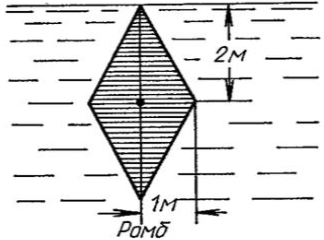
\includegraphics[width=5cm]{images/1a1}

\end{multicols}

\vspace{10mm}

\textbf{Решение.}

\vspace{5mm}

\begin{minipage}{\linewidth}

    \begin{wrapfigure}{r}{0pt}
        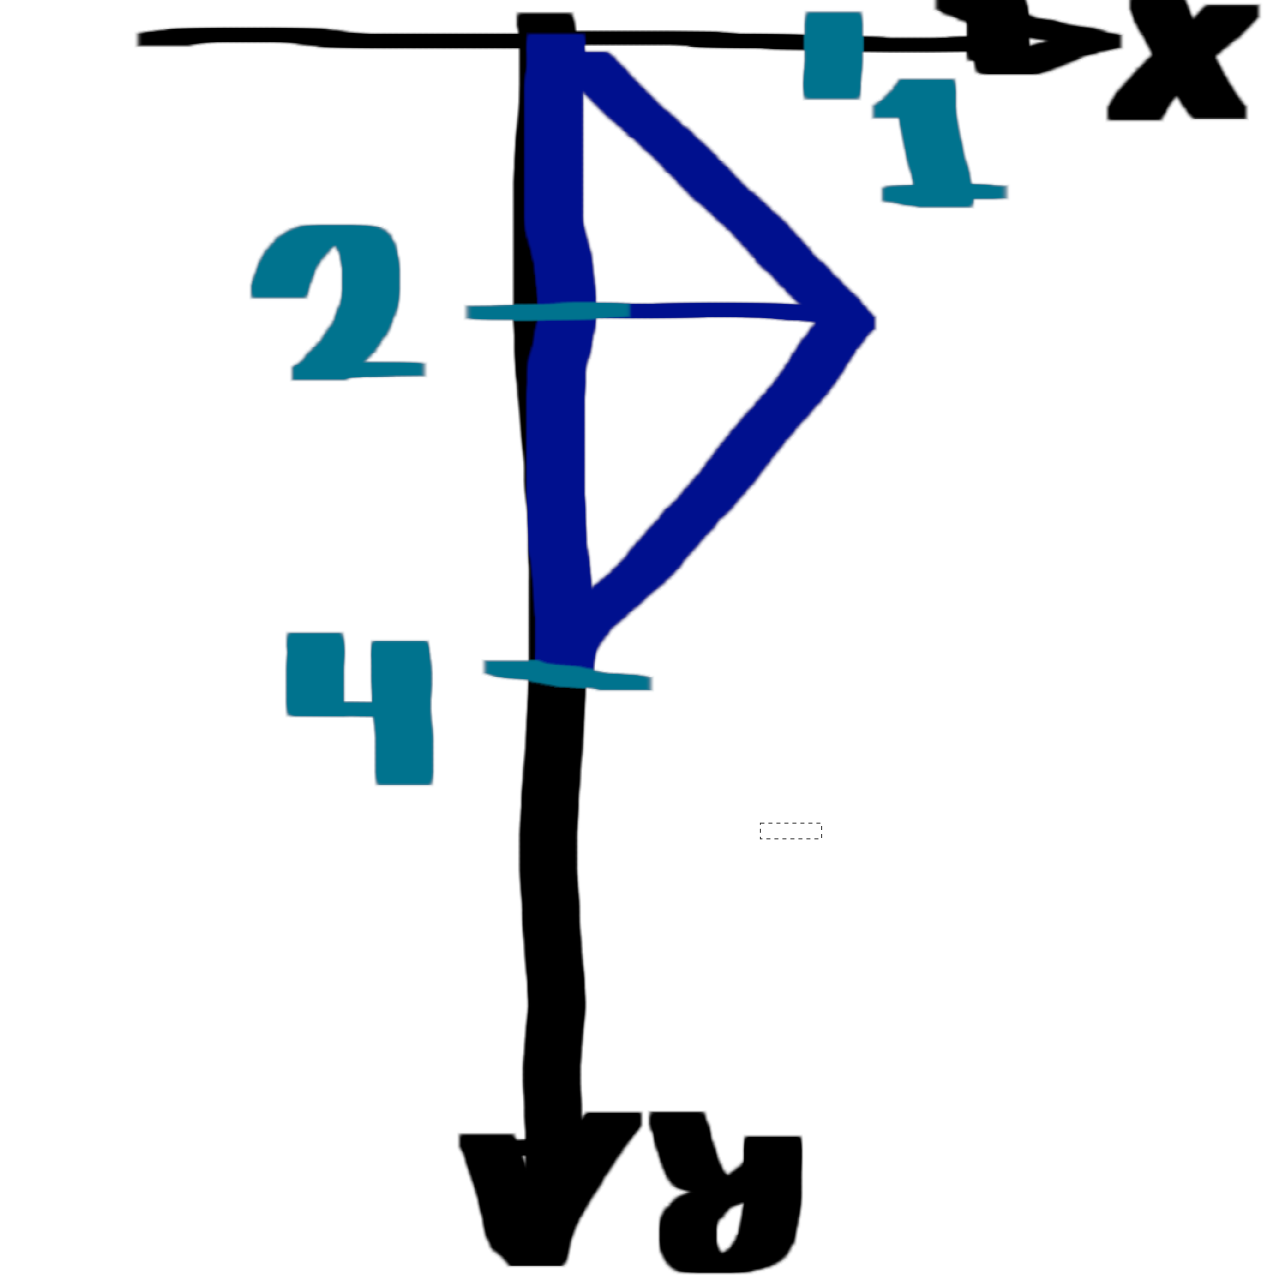
\includegraphics[height=60mm]{images/1a2}
    \end{wrapfigure}

    Сила давления воды вычисляется по формуле: $F = \rho g h$. Т.е. у нас такая задача: есть ромб состоящий из точек и для каждой его точки
    действует функция. И нам нужно вычислить суммарную силу во всех точках. Т.е. взять интеграл. Привяжем начало декартовой системы координат к верхней точке ромба на картинке.
    Ось $Y$ в положительном направлении направим вниз. Тогда у нас есть функция: $f(y) = \rho g y = \gamma y$. Заметим что ромб можно разделить на 2 равных для нашего интеграла треугольника.

\end{minipage}

\vspace{14mm}

Т.е. $\frac{1}{2}$ ответа выглядит так:

\[\iint{f(y)}dxdy = \int_{0}^{2} f(y) dy \int_{x_0 = 0}^{x_1 = 0.5y} dx +
\int_{2}^{4} f(y) dy \int_{x_0 = 0}^{x_1 = 4-0.5y} dx\]
\[ = \int_{0}^{2} f(y)*0.5y dy + \int_{2}^{4} f(y) * (4-0.5y) dy\]
\[ = \int_{0}^{2} \gamma 0.5y^2 dy + \int_{2}^{4} \gamma y * (4 - 0.5y) dy\]
\[ = \int_{0}^{2} \gamma 0.5y^2 dy + \int_{2}^{4} \gamma 4 y - \gamma 0.5y^2 dy\]
\[ = \int_{0}^{2} \gamma d\left(\frac{y^3}{6}\right)  + \int_{2}^{4} \gamma d\left( 2 y^2 - \frac{y^3}{6} \right)\]
\[ = \gamma \left(\frac{2^3}{6} + \left( 2* 4^2 - \frac{4^3}{6} \right) - \left( 2* 2^2 - \frac{2^3}{6} \right) \right)\]
\[ = \gamma \left(\frac{8}{6} + \left( 32 - \frac{64}{6} \right) - \left( 8 - \frac{8}{6} \right) \right)\]
\[ = \gamma \left(\frac{16-64}{6} + 24 \right) = \gamma *\left( 24 - \frac{48}{6}\right) =  \gamma * (24 - 8) =  \gamma * 16 = 156.96\]

Вспомним что это половина ответа: $2 * 156.96 = 313.92$

\textit{Ответ}: $313.92$ Н
\clearpage
